%Kapitel von Mangeng
\ifoot{\mangeng}
\chapter{Projektmanagement}
Damit ein Projekt effektiv initiiert, geplant, abgeschlossen und auch kontrolliert werden kann, wird das Projektmanagement verwendet. Das tatsächliche Ziel hierbei ist es, innerhalb eines bestimmten Zeitplans das Projekt fertigzustellen, dabei die geforderte Qualität zu gewährleisten und auch die vorhandenen Ressourcen, sowohl Personal- als auch Kapitalressourcen, effektiv zu nutzen \cite[vgl.][]{refa:o.J.}.\\
Damit bereits zu Beginn ein grober Überblick über das Projekt vorhanden ist, werden sogenannte Projektpläne erstellt. Die wichtigsten Pläne, welche für diese Diplomarbeit erstellt wurden, werden auf den folgenden Seiten beschrieben.
\section{Projektzieleplan}
In einem Projektzieleplan werden erwartete, messbare Ergebnisse beschrieben und zwischen den folgenden Punkten unterteilt:
\begin{itemize}
	\item \textbf{Haupt-Ziele:} An den Haupt-Zielen wird der  Projekterfolg gemessen. Sie umfassen die Ergebnisse der Diplomarbeit.
	\item \textbf{Neben-Ziele:} Neben- \bzw Zusatz-Ziele sind spezifische Ziele, die zusätzlich neben dem Hauptziel verfolgt werden. Sie können die Qualität eines Produktes erhöhen \bzw den Gesamterfolg des Produktes unterstützen.
	\item \textbf{Nicht-Ziele:} Nicht-Ziele dienen der genaueren Eingrenzung, was in einem Projekt erreicht werden soll. Damit werden Aktivitäten und Prozesse klar ausgegrenzt.
\end{itemize}
Die zu erreichenden Ziele werden meist innerhalb eines Meetings im Team ausgemacht. Treten Veränderungen bei diesen auf, durch beispielsweise Komplikationen, müssen diese Änderungen der Ziele dokumentiert werden \cite[vgl.][]{Diplomarbeiten-bbs:o.J.}. \\ 
Die folgende Tabelle \ref{tab:ziele_plan} beschreibt die Haupt-, Neben- und Nicht-Ziele, die für die Umsetzung dieser Diplomarbeit gelten.
\begin{table}[htpb]
	\caption{Zieleplan}
	\label{tab:ziele_plan}
	\begin{tabular}{p{\dimexpr 0.15\textwidth-2\tabcolsep} | p{0.80\textwidth}}
		\toprule
		\textbf{Zielart} & \textbf{Projektziele} \\
		\midrule
		& Visualisierung der Lüftungsgerät-Werte
		\\
		& Soll parametrierbar ausgeführt werden
		\\
		Hauptziele & Software-Schnittstelle (Zugriff mittels RS323 Schnittstelle)
		\\
		& Kosten in wirtschaftlich sinnvollem Raum
		\\
		& Gehäuse IP66 geschützt 
		\\
		\midrule
		& Nur Werte anzeigen, die auch vorhanden sind (Modbus)
		\\
		& Anleitung für User und Techniker erstellen
		\\
		Nebenziele & Die Anzeige wurde als master definiert. Jetzt sollte sie als Slave definiert werden
		\\
		& Soll QR-Code haben, der beim Scannen die Anzeige am Handy anzeigt
		\\
		\midrule
		& Soll eine Steuerungseinheit darstellen
		\\
		Nichtziele & Benutzerverwaltungsmöglichkeit
		\\
		& Bildschirm- und Bediensperre
		\\
		\bottomrule
	\end{tabular}
\end{table}

\newpage
\newpage
\section{Projektumweltanalyse}
Damit in einem Projekt Veränderungen und Entwicklungen in Umwelten frühzeitig erkannt werden können, um richtig reagieren zu können, werden Umweltanalysen angefertigt. Hier werden die Umfelder nach verschiedenen Kriterien analysiert, die das Unternehmen auf eine gewisse Art beeinflussen. Das tatsächliche Ziel ist es, eine Übersicht über die Umwelten zu haben, um Handlungsempfehlungen ausgeben zu können. Im Marketing wird zwischen internen und externen Faktoren unterschieden \cite[vgl.][]{wikipedia:2023, marketing:2024}.

\section{Projektorganigramm}
Ein Projektorganigramm ist ein wichtiges Instrument zur Darstellung der internen Struktur und der wechselseitigen Beziehungen innerhalb eines Projektteams. Es ermöglicht einen klaren Überblick über die verschiedenen Rollen und Verantwortlichkeiten der Mitarbeiter, sowie deren Hierarchieebenen und deren jeweilige Berichtswege \cite[vgl.][]{projektmanagement-definitionen:2009}. \\
Die folgende Abbildung \ref{fig:organigramm} stellt die existierende, interne Struktur der Diplomarbeit dar, welche daraufhin in der Tabelle \ref{tab:projektorganisation} deutlicher beschrieben wird.

\begin{figure}[H]
	\centering
	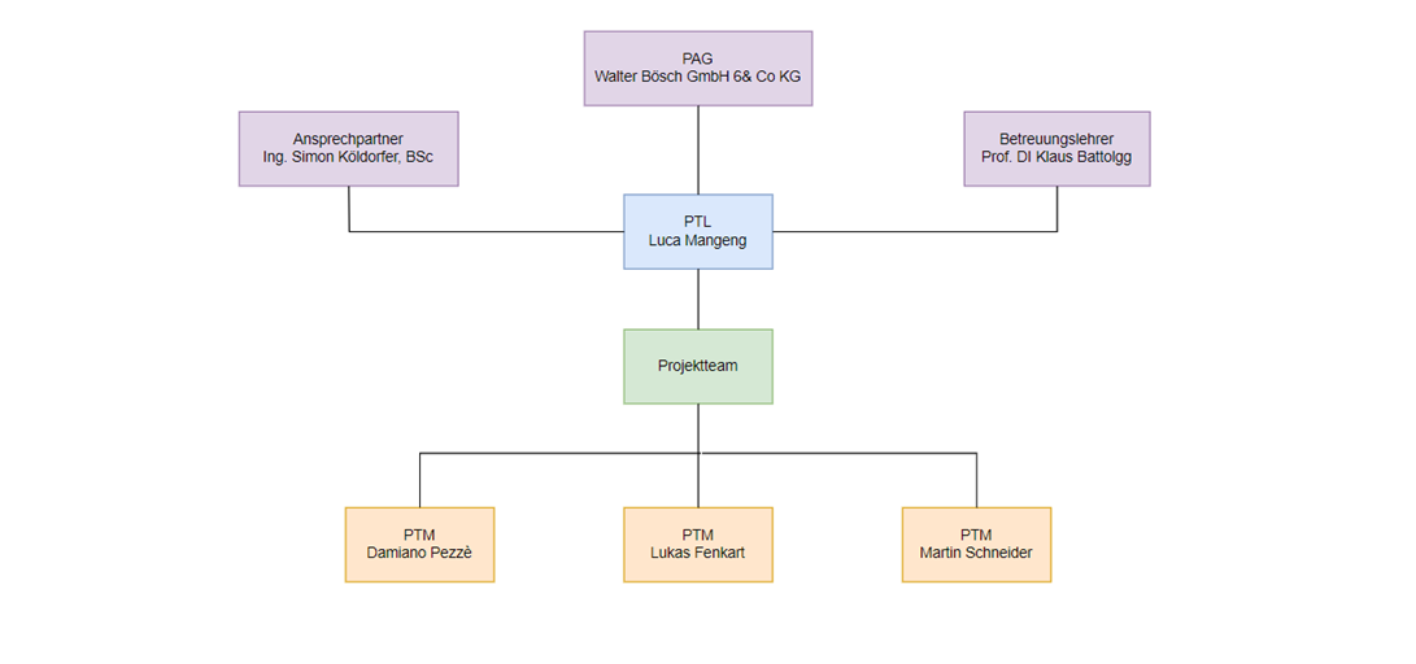
\includegraphics[width=1\linewidth]{Bilder/Organigramm}
	\caption{Projektorganigramm}
	\label{fig:organigramm}
\end{figure}

\begin{table}[H]
	\caption{Projektorganisation}
	\label{tab:projektorganisation}
	\begin{tabular}{p{\dimexpr 0.25\textwidth-2\tabcolsep} | p{0.50\textwidth} | p{0.20\textwidth}}
		\toprule
		\textbf{Projektrolle} & \textbf{Aufgabenbereich/Skills} & \textbf{Name} \\
		\midrule
		Projektauftraggeber & Gibt den Auftrag für die Universalananzeige und setzt Bedingungen und Ziele, die im Projekt erreicht werden sollen. Auch setzt er eine Fertigstellungsfrist & Walter Bösch GmbH \& Co. KG
		\\
		\midrule
		Projektleiter & Leitung des Projekts;
		Verantwortlich für die Einhaltung der Fertigstellung des Projekts und für die Einhaltung der Bedingungen; Hilft bei der Programmierung, dem Aufbau der Hardware den Berechnungen und Tests
		 & Luca Mangeng
		\\
		\midrule
		Projektteam-mitglieder & Zuständig für die Erstellung des Codes, Zusammenstellung und Zusammenbau der preiseffizienten Hardware & 
		\fenkart, \pezze, \schneider
		\\
		\bottomrule
	\end{tabular}
\end{table}

\section{Projektstrukturplan}
Der Projektstrukturplan zeigt hierarchisch gegliedert alle plan- und kontrollierbaren Teilaufgaben. Diese Teilaufgaben entstehen dadurch, indem die Gesamtaufgabe des Projektes so lange in kleinere Arbeitspakete aufgeteilt wird, bis eine weitere Aufteilung nicht mehr sinnvoll wäre. Durch die hierarchische Struktur entstehen Ebenen, in die das Projekt aufgeteilt ist. Die oberste Ebene ist die Allgemeinheit des Projekts, betitelt mit dem Projektnamen. Darunter befinden sich die Phasen und unter diesen befinden sich besagte Arbeitspakete. Jeder dieser Punkte hat seinen eigenen, eindeutigen PSP-Code.
\\Der \enquote{PSP} stellt auch die Grundlage für weitere relevante Planungsschritte im Projektmanagement dar, wie beispielsweise Terminpläne, Ressourcenpläne und Kostenpläne \cite{Kindl_Niels:2023}.

\begin{figure}[H]
	\centering
	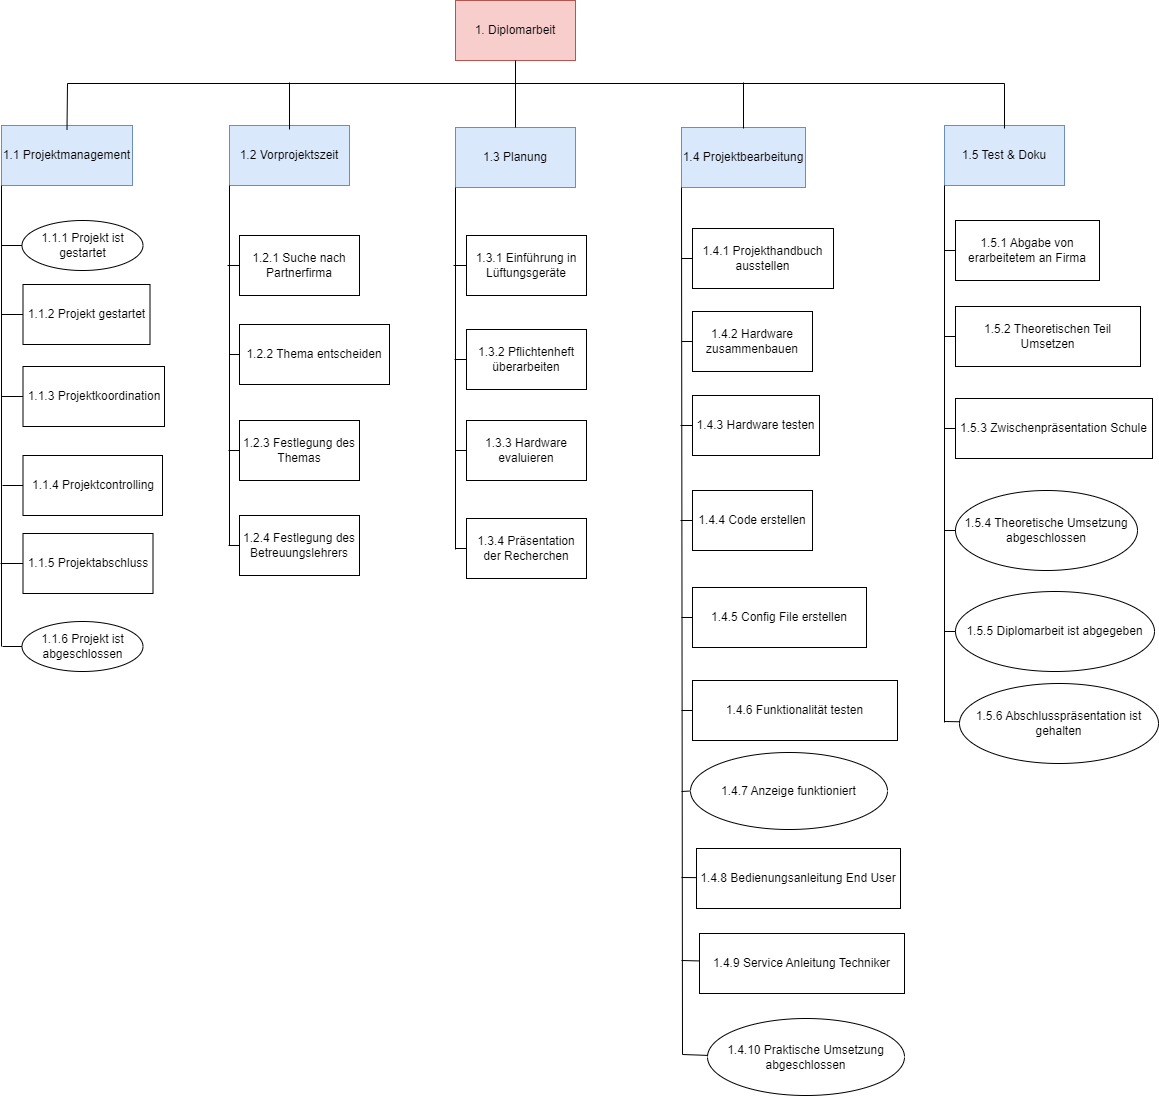
\includegraphics[width=1\linewidth]{Bilder/projektstrukturplan}
	\caption{Projektstukturplan}
	\label{fig:projektstrukturplan}
\end{figure}

\section{Objektstrukturplan}
Ein Objektstrukturplan wird am Anfang eines Projekts definiert. Dieser ist dafür zuständig, zu zeigen, welche Ergebnisse und Zwischenergebnisse im Projekt entstehen sollen. Dabei können diese sowohl materiell als auch immateriell sein. Der \enquote{OSP} hat keine zeitliche Abfolge und soll bei der Ausarbeitung des Projektstrukturplans helfen. Die Darstellung kann als Mindmap, aber auch als Baum- oder Listenstruktur erfolgen.

\section{Projektfunktionendiagramm}
Um die Zuständigkeiten in Projekten regeln zu können, existieren Projektfunktionendiagramme. Diese werden in Form einer Tabelle dargestellt und beinhalten alle Projektbeteiligten sowie alle Arbeitspakete. Bei den Beteiligten gelten folgende Kürzel:
\begin{itemize}
	\item \textbf{PAG} - Projektauftraggeber
	\item \textbf{PL} - Projektleiter
	\item \textbf{PTM} - Projektteammitglied
	\item \textbf{PM} - Projektmitarbeiter
\end{itemize}
Unter jedem Beteiligten sind die jeweiligen Funktionen dessen eintragbar, die bei der Ausführung des Arbeitspakets eingenommen wurde.
Bei den Funktionen gelten folgende Kürzel:
\begin{itemize}
	\item \textbf{D} - Durchführungsverantwortung
	\item \textbf{M} - Mitarbeit
	\item \textbf{I} - bekommt Informationen
\end{itemize}
Hier ist zu beachten, dass die Verantwortung eines Arbeitspakets nur durch eine Person übernommen werden kann \cite{prezi:o.J.}.

\section{Projektmeilensteinplan}
Zur Überprüfung, ob ein Projekt möglicherweise nicht zur richtigen Zeit beendet wird, kann der Meilensteinplan als Maßstab dienen. Er bildet die wichtigsten Ereignisse inklusive einer Deadline ab. So erhält man eine grobe Übersicht über Verzögerungen und es können Maßnahmen bei Bedarf ergriffen werden. Im Allgemeinen dient er aber auch der Mitarbeitermotivation bei Erreichen eines Zwischenziels oder Meilensteins \cite[vgl.][]{domendos:2016}. \\
In der folgenden Tabelle \ref{tab:meilensteinplan} befinden sich die Meilensteine inklusive deren Termine.

\begin{table}[H]
	\caption{Projektmeilensteinplan}
	\label{tab:meilensteinplan}
	\begin{tabular}{p{\dimexpr 0.10\textwidth-2\tabcolsep} | p{0.30\textwidth} | p{0.15\textwidth} | p{0.15\textwidth} | p{0.15\textwidth}}
		\toprule
		\textbf{PSP-Code} & \textbf{Meilenstein} & \textbf{Basis-Termine} & \textbf{Aktuelle Plantermine} & \textbf{Ist Termine} \\
		\midrule
		1.1.1 & M1 Projekt ist gestartet & 09.05.2023 & 09.05.2023 & 09.05.2023 \\
		\midrule
		1.4.7 & M2 Anzeige funktioniert & 02.08.2023 & 03.08.2023 & 03.08.2023 \\
		\midrule
		1.4.10 & M3 Praktische Umsetzung abgeschlossen & 03.08.2023 & 04.08.2023 & 04.08.2023 \\
		\midrule
		1.5.4 & M4 Theoretische Umsetzung abgeschlossen & 01.03.2024 & 01.03.2024 & 01.03.2024 \\
		\midrule
		1.5.5 & M5 Diplomarbeit ist abgegeben & 03.04.2024 & 03.04.2024 & 03.04.2024 \\
		\midrule
		1.5.6 & M6 Abschlusspräsentation ist gehalten & 13.06.2024 & 13.06.2024 & 13.06.2024 \\
		\midrule
		1.6 & M8 Projekt ist abgeschlossen & 13.06.2024 & 13.06.2024 & 13.06.2024 \\
		\bottomrule
	\end{tabular}
\end{table}


\section{Projektbalkenplan}
Während bei dem Meilensteinplan nur die Meilensteine abgebildet sind, werden im Projektbalkenplan alle Arbeitspakete und deren ungefähres Fälligkeitsdatum gezeigt. So hat man jederzeit einen Überblick über den terminlichen Status des Projektfortschritts. Daher ist der Projektbalkenplan oder \enquote{Gantt-Chart}  als zeitliche Ebene die erste Wahl, um einen umfassenden Überblick über den zeitlichen Status des Projektfortschritts zu behalten \cite[vgl.][]{domendos:2019}. \\
Auf der nächsten Seite befindet sich mit Abbildung \ref{fig:projektbalkenplan} der Balkenplan, der nach dem \enquote{PSP} aufgebaut ist.

\begin{landscape}
	\begin{figure}[H]
		\centering
		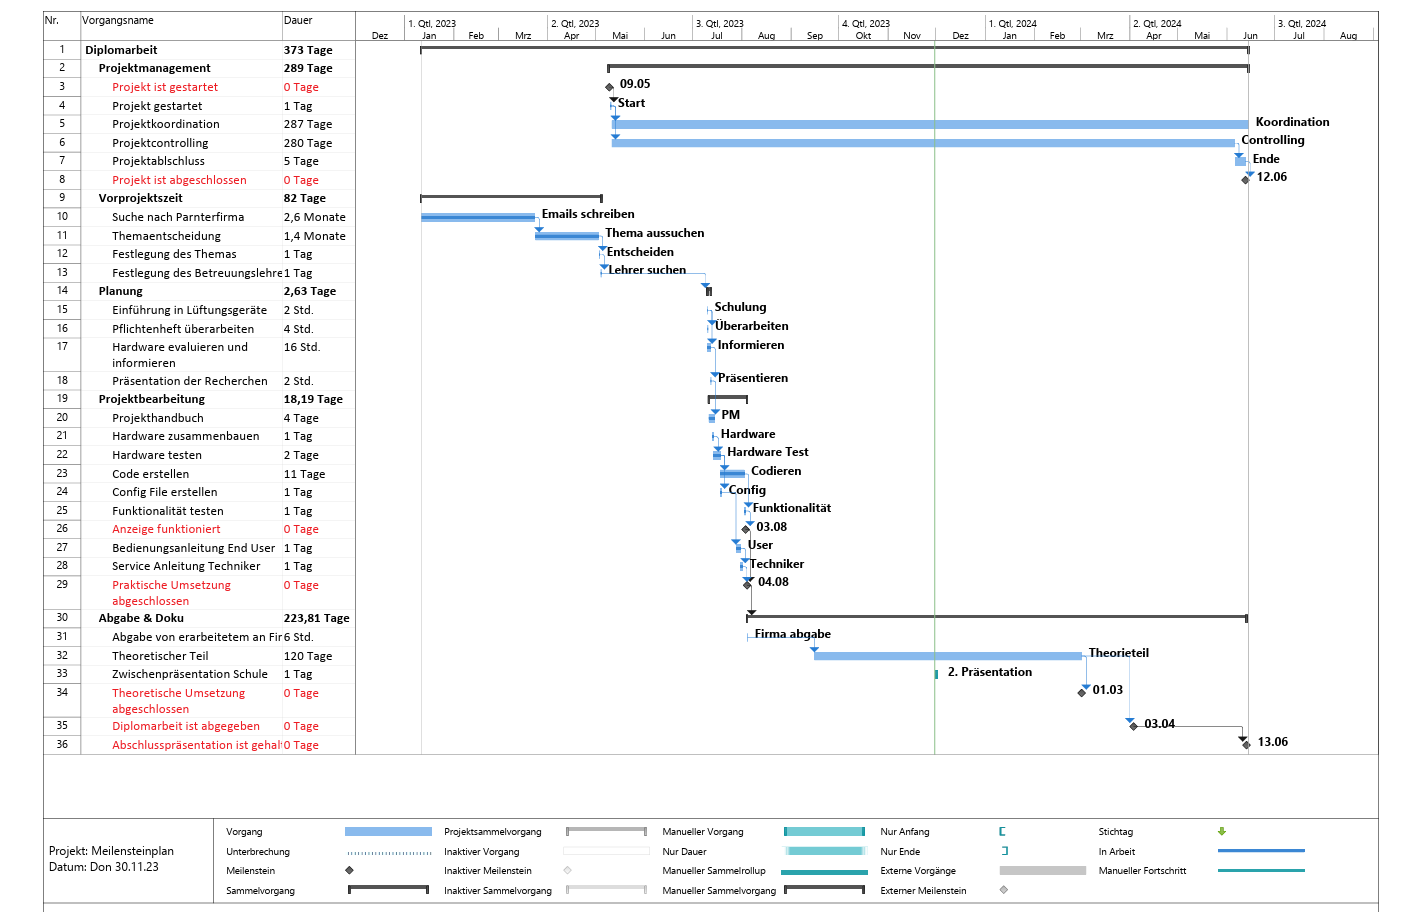
\includegraphics[width=1\linewidth]{Bilder/ganttchart}
		\caption{Projektbalkenplan}
		\label{fig:projektbalkenplan}
	\end{figure}
\end{landscape}

\section{Projektrisikoanalyse}
Risiken können in den meisten Fällen ein Projekt bedrohen. Daher ist es wichtig, Risiken im Vorhinein einzuschätzen und möglichst zu vermeiden. Manche Risiken können teilweise nicht umgangen werden, dafür, wenn das Risiko überwunden wurde, stärkt es das Projekt durch diese Herausforderung. Dennoch sollten diese immer zuvor bereits bemerkt werden, damit der Zeitaufwand mit einberechnet werden kann \cite{timetrackapp:2021}.

\begin{longtable}{p{\dimexpr 0.10\textwidth-2\tabcolsep} | p{0.20\textwidth} | p{0.20\textwidth} | p{0.10\textwidth} | p{0.10\textwidth} | p{0.20\textwidth}}
	\caption{Projektrisikoanalyse}
	\label{tab:risikoanalyse}
	\\ \toprule
	\textbf{PSP-Code} & \textbf{AP-Bezeichnung} & \textbf{Risiko-beschreibung} & \textbf{Prio} & \textbf{Verzö-gerung} & \textbf{korrektive Maßnahmen}
	\\ \midrule
	\endfirsthead
	\caption{Projektrisikoanalyse (Fortsetzung)}
	\\ \toprule
		\textbf{PSP-Code} & \textbf{AP-Bezeichnung} & \textbf{Risiko-beschreibung} & \textbf{Prio} & \textbf{Verzö-gerung} & \textbf{korrektive Maßnahmen}
	\\ \midrule
	\endhead
	%
	\midrule
	\multicolumn{6}{r}{{Auf nächster Seite weitergeführt}} 
	\\ \bottomrule
	\endfoot
	%
	\bottomrule
	\endlastfoot
	1.3.3 & Hardware evaluieren &  Für eine zu lange Zeit keine passenden Komponenten und keine Informationen für die Umsetzung finden & 1 & 1 Tag & Zu Beginn viel Zeit in das Recherchieren investieren und wichtige Informationen für später herausschreiben \\ \midrule
	1.4.2 & Hardware zusammenbauen & Möglicherweise passen die Teile nicht zusammen bzw. sind für andere Versionen des Chipsatzes gedacht & 2 & 3 Tage & Exzessiv auf die Informationen, die auf den Websites der Bauteile stehen, achten  \\ \midrule
	1.4.3 & Hardware testen & Defekte Komponente & 3 & 3 Tage & Neue Hardware muss bestellt werden \\ 
	1.4.4 & Code erstellen & Probleme bei der Programmierung der Modbus-Schnittstelle oder dem Anzeigen der Daten auf dem Display & 1 & 2 Tage & Vor dem Programmieren informieren und nach Libraries suchen, die die Einstellungen vereinfachen \\ \midrule
	1.4.4 & Code erstellen & Anforderungen von Arbeitgeber anders gewünscht als tatsächlich erledigt & 4 & 3 Tage & Klares absprechen, was im Projekt behandelt wird und auch wie \\ \midrule
	1.4.6 & Funktionalität testen & Mögliche weitere Anforderungen des Arbeitgebers nach eigentlicher Beendigung des Projekts  & 4 & 3-4 Tage & Durch ein klar definiertes und unterschriebenes Pflichtenheft müssen nur vorher besprochene Themen bearbeitet werden \\
\end{longtable}

\section{Projektkommunikationsstrukturen}
Neben der Erstellung von Plänen und Analysen ist der Projektleiter auch noch für die Projektkoordination und das Projektcontrolling zuständig. Dies gilt demnach natürlich auch für Meetings, die intern im Unternehmen für die Ausarbeitung der Diplomarbeit stattfanden. Die folgende Tabelle \ref{tab:strukturenplan} beinhaltet alle Treffen und Meetings inklusive Datum. \\
Stattgefunden hat alles bei der Firma Bösch in Lustenau, mit dem Projektansprechpartner Simon Köldorfer sowie allen Projektmitgliedern als Teilnehmern, abgesehen vom letzten Meeting, welches an der HTL Dornbirn stattfand mit Beisitz von Herrn Battlogg.

\begin{table}[H]
	\caption{Projektkommunikationsstrukturenplan}
	\label{tab:strukturenplan}
	\centering
	\begin{tabular}{p{\dimexpr 0.25\textwidth} | p{0.45\textwidth} | p{0.15\textwidth}}
		\toprule
		\textbf{Bezeichnung} & \textbf{Ziele, Inhalt} & \textbf{Termin} \\
		\midrule
			& • Diskussion Projektablauf & \\
		      Projektauftraggeber - &  • Besprechung Pflichtenheft  & 02.05.2023 \\
 			 Sitzung & • Freigabe Projektfortschrittsbericht & \\
 		\midrule
 			& • Fachspezifisches Personal kennen & \\
 		    Kennenlernen des & • Einführung in die Lüftungstechnik & 10.05.2023 \\
 			Personals	& • Ansprechperson bei Fragen & \\
 			& • Fragen zu Beginn geklärt & \\
 		\midrule
 			& •	Projektstatus & \\
 			& •	Hardware Möglichkeiten zeigen & \\
 		    Hardware -	& • Kosten, Ressourcen & 12.07.2023 \\ 
 			Präsentation & • Diskussion Problemstellungen & \\
 			& • Diskussion Lösungswege & \\
 			& •	Controlling Leistungsfortschritt & \\
 		\midrule
 			& •	Projektstatus & \\
 		Besprechung der & •	Design-Möglichkeiten & 27.07.2023 \\
 		anzuzeigenden Werte & •	Gewünschte Anzeigewerte besprechen & \\
 			& • Aufbau des Programms  & \\
 		\midrule
 			& •	Was ist abzugeben & \\
 		Weitere Schritte & • Vorhandene Probleme & 04.08.2023 \\
 			& •	Projektvorführung & \\
 			& •	Erklärung von Config Files & \\
 		\midrule
 			& •	Übergabe eines Gehäuseprototypen & \\
 		Tag der offenen Tür & • Gespräch über Möglichkeiten für die Präsentation & 09.11.2023 \\
 			& •	Besorgung von Hardware seitens Herrn Köldorfer& \\
		\bottomrule
	\end{tabular}
\end{table}

